% !TEX root = ../main.tex

\chapter{Practical Implementation}
\label{ch:practical}

\emph{Part of this research has been described in a journal article in Digital Creativity in 2013, and I presented a paper at the Creativity and Cognition conference 2013 in Sydney.}

\grule

\section{User experience}

Whilst developing a system that returns creative results to the end user has numerous advantages, the assumptions that are made about and the decisions we take for the user must still be considered. For example, presume that the user inputs a search request 'The Cat in the Hat' after reading a Dr. Seuss book to their child, and the system employs an anomalous method on the query and searched 'sunglasses'. Whilst there is logic to the new search request, it is anomalous to the initial request, if the user receives these results without being told what method was used, the results will appear random, and therefore are likely to be detrimental to the user. Therefore the level of interaction the user has with the system and the feedback the system gives to the user on decisions it is making will have a large influence on the overall effectiveness and appreciation of the search tool. A quick and simple solution to this problem would be to add an icon to the side of each search result which displays how the original query was pataphysicalised.

\begin{figure}[htb] % (here, top, bottom, page)
  \centering
  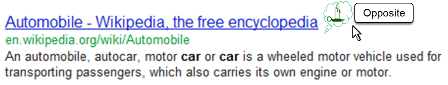
\includegraphics[width=\linewidth]{images/resultexample}
\caption[Feedback button]{Feedback button}
\label{fig:feedback}
\end{figure}

The above image (figure 3) shows an example of how this could be implemented. The little green candle (a reference to pataphysics in itself by the way) shows a pop-up note when hovered over with the mouse pointer. In this case the original query could have been ‘tree’ and ‘car’ was returned as an opposite to that.

In the end, it comes to a point of being able to identify which of these factors will affect how the user perceives the results and which do not, and therefore give the system greater flexibility. This in itself is a huge undertaking, with which large quantities of empirical data will be required and is therefore left for future work on the project.

\section{Algorithms}

\begin{table}[htb]
  \begin{tabu}{X[1]|X[3]X[3]X[2]}
  \toprule
  % \cline{2-4}
  &
  \textbf{clinamen}
  &
  \textbf{syzygy}
  &
  \textbf{antinomy}
  \\ \midrule
  \textbf{clear}
  &
  altar, leaf, pleas, cellar
  &
  vanish, allow, bare, pronounce
  &
  opaque
  \\ \midrule
  \textbf{solid}
  &
  sound, valid, solar, slide
  &
  block, form, matter, crystal, powder
  &
  liquid, hollow
  \\ \midrule
  \textbf{books}
  &
  boot, bones, hooks, rocks, banks
  &
  dialogue, authority, record, fact
  &
  -
  \\ \midrule
  \textbf{troll}
  &
  grill, role, tell
  &
  wheel, roll, mouth, speak
  &
  -
  \\ \midrule
  \textbf{live}
  &
  love, lies, river, wave, size, bite
  &
  breathe, people, domicile, taste, see, be
  &
  recorded, dead
  \\ \bottomrule
  \end{tabu}
\caption[Comparison of algorithms]{Comparison of algorithms}
\label{algorithmscomp}
\end{table}

\subsection{Clinamen}

The clinamen is the unpredictable swerve that Bök calls "the smallest possible aberration that can make the greatest possible difference" (Bök 2002).

The clinamen function uses the Damerau-Levenshtein algorithm [10], which measures the distance between two strings (with 0 indicating equality), to find words that are similar but not quite the same. The distance is calculated using insertion, deletion, substitution of a single character, or transposition of two adjacent characters. This means that we are basically forcing the program to return matches that are of distance two or one, meaning they have two or one spelling errors in them (see Eq. (1)). While we only return matches that actually appear in the book (i.e. they exist in the index), and by doing so eliminate the introduction of new words like Jarry's merdre, the swerve or aberration is still evident.

\begin{lstlisting}
  Clinamen(t):
    matches = {v : 0 < dameraulevenshtein(t, v) <= 2},   for v $\in$ V
    return matches
\end{lstlisting}

Line 1 of the algorithm above creates a set of matches, where each match is a word v from our vocabulary V if the Damerau-Levenshtein function computed with query term t returns a value less than or equal to 2 but higher than 0 (not the query term itself).

\begin{equation}
  clinamen(t) = [v \colon 0 < dameraulevenshtein(t,v) \leq 2] \ \text{for} \ v \in V
\label{eq:clinamen}
\end{equation}
\myequations{clinamen}

\subsection{Syzygy}

The syzygy surprises and confuses. It originally comes from astronomy and denotes the alignment of three celestial bodies in a straight line. In a pataphysical context it is the pun. It usually describes a conjunction of things, something unexpected and surprising. Unlike serendipity, a simple chance encounter, the syzygy has a more scientific purpose.

For the syzygy function, we made use of WordNet [29] through the NLTK python library [26] to find suitable results. Specifically, as shown in Eq. (2), the algorithm fetches the set of synonyms (synsets) first and then finds any hyponyms, hypernyms or holonyms for each of those (each of which denotes some sort of relationship or membership with its parent synonym). This mimics the syzygy alignment of three words in a line mentioned earlier (query $\to$ synonym $\to$ hypo/hyper/holonym).

This algorithm makes heavy use of WordNet. Line 1 creates a set of all synonyms for query term t from WordNet. It then loops through all individual items in the list of synonyms in line 2 to 5. Line 3 adds all hyponyms h for the current synonym s if there exists a word in the vocabulary same as the hyponym. Similarly lines 4 and 5 add all hypernyms and holonyms to the results list which is then returned in line 6.

\begin{lstlisting}
  Syzygy( t ):
    synonyms = { s $\in$ WordNet-synsets( t ) }
    for each s in synonyms:
      hypo   = { h : h $\in$ WordNet-hyponyms( s ) }
      hyper = { h : h $\in$ WordNet-hypernyms( s ) }
      holo    = { h : h $\in$ WordNet-holonyms( s ) }
      union = hypo $\cup$ hyper $\cup$ holo
      add { h : h $\in$ union and $\exists$ h $\in$ V } to results
    return results
\end{lstlisting}

\begin{equation}
\begin{split}
  syzygy(t) &= \{ h \colon h \in union(t) \ \text{and} \ \exists \ h \in V \}\\
  union(t) &= hypo(t) \cup hyper(t) \cup holo(t)\\
  hypo(t) &= \{ h \colon h \in hyponyms(s) \}, \text{for} \ s \in syno(t)\\
  hyper(t) &= \{ h \colon h \in hypernyms(s) \}, \text{for} \ s \in syno(t)\\
  holo(t) &= \{ h \colon h \in holonyms(s) \}, \text{for} \ s \in syno(t)\\
  syno(t) &= \{ s \colon s \in synonyms(t) \}
\end{split}
\label{eq:syzygy}
\end{equation}
\myequations{syzygy}

\subsection{Antinomy}

The antimony, in a pataphysical sense, is the mutually incompatible.

For the antinomy we simply used WordNet’s antonyms (opposites) (see Eq. (3)). This function exhibits the same problem as mentioned above for the syzygy, just much worse.  Arguably, some words just do not appear to have an opposite, but the pataphysical antinomy should still be able to find a match. A better thesaurus or a larger index (e.g. based on more than one book – or, of course, the Web) could improve this method.

This algorithm is very similar to the algorithm for the syzygy. It finds all antonyms through WordNet and returns them if they appear in our dictionary of words.

\begin{lstlisting}
  Antinomy(t):
    synonyms = { s $\in$ WordNet-synsets(t) }
    for each s in synonyms:
      add { h $\in$ WordNet-antonyms(s) : $\exists$ h $\in$ V } to results
    return results
\end{lstlisting}

\begin{equation}
  \begin{split}
  antinomy( t ) &= \{ h \colon h \in anto( t ) \ \text{and} \ \exists \ h \in V \}\\
  anto( t ) &= \{ h \colon h \in antonyms( s ) \}, \text{for} \ s \in syno( t )\\
  syno( t ) &= \{ s \colon s \in synonyms( t ) \}
  \end{split}
\label{eq:antinomy}
\end{equation}
\myequations{antinomy}

\section{Implementation}

\begin{comment}
  Interface (first tier) – application (second tier) – database/corpus (third tier)
\end{comment}

The general concept of the project described in this paper is pataphysical web searching and the following three points summarize its main aims:

\begin{itemize}
  \item search the Web for suitable answers to a given query,
  \item return results as a list or a mixture of data structures, and
  \item present pataphysical results (rather than relevant ones).
\end{itemize}

The essence of the proposed search tool lies in its algorithms which make the difference to traditional search engines. The philosophical ideology behind the tool is fundamentally different. Our system will still consist of the main components typically found in Web search engines (crawler, index and ranking) but they will have slightly different inner workings and target a different audience of users.

To link back to some of the creative, pataphysical concepts we have discussed earlier, let us put some of the ideas for our tool into perspective. The constraints for our conceptual space are the pataphysical rules that we want to apply to our data. We use those rules to explore, combine and transform our space; giving us the flexibility and freedom we need to find interesting results.

We developed the idea of pataphysicalising data as the process of applying such pataphysical rules in order to produce creative search results. This pataphysicalisation process forms a central component of our system (see Figure \ref{fig:patasearch01}) and influences all areas of the search tool.

Our index will contain what Hendler and Hugill have called patadata [15].  Patadata is to metadata as metadata is to data - inspired by one of the definitions of pataphysics: that which is above that which is after physics [20]. This suggests that patadata provides another layer of information above information.  If metadata helps us organise information semantically then patadata is for organising information pataphysically. If metadata is objective then patadata is subjective and that is precisely what pataphysics is for.

\todo{redraw figure}

\begin{figure}[htb] % (here, top, bottom, page)
  \centering
  
\includegraphics[width=\linewidth]{images/patasearch01}
\caption[Pata central]{Pata central}
\label{fig:patasearch01}
\end{figure}

\begin{figure}[htb] % (here, top, bottom, page)
  \centering
  % \def\svgwidth{\columnwidth}
  \input{images/patasearch01.pdf_tex}
\caption[Pata central]{Pata central}
\label{fig:patasearch01}
\end{figure}

The prototype described here (see Figure 2) was developed as a proof-of-concept tool to demonstrate some example search results using pataphysical algorithms.

It is by no means a fully functioning Web search engine, in fact it does not search the Web at all, and only the main algorithmic functionality is discussed here. The tool searches the text of an example book, namely Alfred Jarry’s Exploits and Opinions of Dr. Faustroll, Pataphysician [20].

In short, the prototype’s workflow can be described as follows:
\begin{itemize}
  \item tokenise text and remove stopwords to build index,
  \item query triggers the three pataphysical functions,
  \item each function finds matches for query as described above,
  \item retrieve some words before/after match for context, and
  \item return list of resulting sentences.
\end{itemize}

The three functions inspired by pataphysics (clinamen, syzygy and antinomy) are described in more detail in the previous section. Figure 2 shows a screenshot of the resulting list of results for the query clear. The specific results for each of the three methods are simply a few words surrounding the pataphysicalised query term from within the book, which does not necessarily represent complete sentences but provides some context for the result.

The same principles and algorithms can be applied to different types of media, for example images or video and even sound. The complete tool would include a mixture of different types of media in its results with various styles of displaying them (e.g. displaying images ordered as a Fibonacci spiral).

\subsection{Prototype 1}

\begin{figure}[htb] % (here, top, bottom, page)
  \centering
  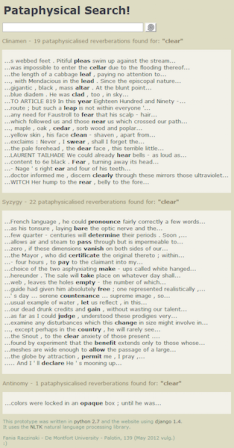
\includegraphics[height=0.6\textheight]{images/prototype01}
\caption[Prototype1]{Prototype1}
\label{fig:Prototype1}
\end{figure}

\subsection{Prototype 2}

\begin{figure}[htb] % (here, top, bottom, page)
  \centering
  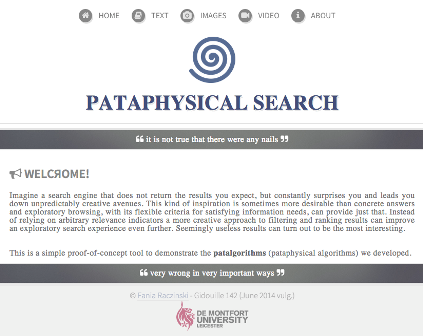
\includegraphics[width=\linewidth]{images/prototype02}
\caption[Prototype2]{Prototype2}
\label{fig:Prototype2}
\end{figure}

\begin{alltt}
# TEXT

## setup

1. read in faustroll book
2. create `froll_dict` dictionary from text
3. remove stopwords and numbers from `froll_dict`

## text algorithm

1. get query term
2. execute three functions:

  2a. syzygy algorithm
    1. get list of synonyms
    2. for each synonym do the following:
      a. find hyponyms; if a hyponym occurs in `froll_dict` then add to the output list
      b. find hypernyms; if a hypernym occurs in `froll_dict` then add to the output list
      c. find holonyms; if a holonym occurs in `froll_dict` then add to the output list
    3. return list of syzygy words

  2b. antinomy algorithm
    1. get list of synonyms
    2. for each synonym do the following:
      a. find antonyms; if a antonym occurs in `froll_dict` then add to the output list
    3. return list of antinomy words

  2c. clinamen algorithm
    1. find list of words within `froll_dict` that have a `dameraulevenshtein distance` of 1 or 2 (meaning, there are 1 or 2 spelling errors)
    2. return list of clinamen words

3. get sentences for all three output lists

  3a. if the word appears in faustroll then find the nearest 5 words before and after the word
  3b. return list of sentences

4. render results as html


---

# IMAGES

## setup

- microsoft translate API key
- flickr API key
- (bing image search API key) - not used atm

## image algorithm

1. get query word
2. get one syzygy word using syzygy algorithm 2a above
3. translation party
  3a. translate english to french
  3b. translate french to japanese
  3c. translate japanese to english
4. get images
  4a. search flickr for 10 matches to english translation
  4b. get metadata for each
  4c. add title, thumb, link to output list
5. return output list
6. render results as html

---

# VIDEOS

## setup

- microsoft translate API key
- youtube API stuff
- (bing video search API key) - not used atm

## video algorithm

1. get query word
2. get one syzygy word using syzygy algorithm
3. translation party
  3a. translate english to french
  3b. translate french to japanese
  3c. translate japanese to english
4. get videos
  4a. search YouTube for 10 matches to english translation
  4b. get metadata for each
  4c. add title, thumb, link to output list
5. return output list
6. render as html
\end{alltt}


\section{Website}

\url{http://pata.fania.eu}

\section{APIs}

\begin{itemize}
  \item Bing
  \item YouTube
  \item Microsoft Translate
  \item Flickr
  \item WordNet
\end{itemize}

\section{Design}

\begin{itemize}
  \item random sentences
  \item spiral
  \item Word Scrable
  \item $\dots$
\end{itemize}
